\section{Introduction}
\label{sec:introduction}

% state the learning objective
\par The objective of this laboratory assignment is to study a RC circuit functioning in two diferent regimes: stationary and transient. The frequency response of the circuit is also studied. The circuit to be analysed is composed of seven resistors, two voltage sources, one independent and one controlled by current, one current source controlled by voltage, and one capacitor. The results of the theoretical analysis will be compared with a computational simulation. The given circuit can be seen in Figure~\ref{fig:circuit}.

\begin{figure}[H]
\centering
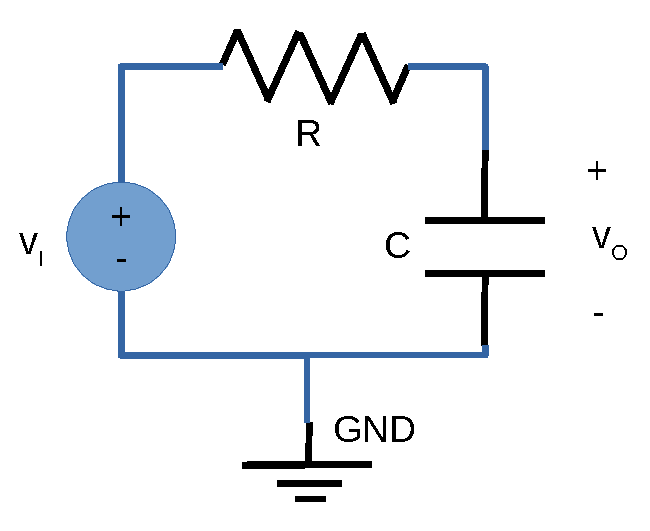
\includegraphics[width=10 cm]{rc.pdf}
\caption{RC circuit to be studied}
\label{fig:circuit}
\end{figure}

\begin{multicols}{2}
\begin{equation}
    v_s(t) = V_s u(-t) + sin(2 \pi ft) u(t)
    \label{eq:v_s}
\end{equation}

\begin{equation}
    u(t) = \left \{ \begin{matrix} 0, & t<0 \\ 1, & t\geqslant 0 \end{matrix} \right.
    \label{eq:u}
\end{equation}
\end{multicols}

\par In Section~\ref{sec:analysis}, a theoretical analysis of the circuit is presented in which, with the help of \textit{Octave} software, we aim to analyse the system  in $t<0$ at a stationary regime, in $t=0$ and its time evolution in $t>0$, namely the 6th and 8th node's voltages, as well as the capacitor's.
Looking to equations \ref{eq:v_s} and \ref{eq:u}, one can easily see that the circuit will perform in a different regime after time $t=0$, because $v_s$ is the only independent source in the circuit. We also do a frequency analysis in $t>0$, to see how would the voltage amplitudes of the nodes (and components) and its phases change
with respect to the voltage source's frequency. This theoretical analysis is strongly based on the nodal method.

\par In Section~\ref{sec:simulation}, the circuit is analysed by
simulation, using the software \textit{ngspice}, and the results are compared to the theoretical results obtained in
Section~\ref{sec:analysis}. The conclusions of this study are outlined in Section~\ref{sec:conclusion}.
